\documentclass[11pt,UTF8]{ctexart}
\usepackage{titling}
\usepackage{enumerate}
\usepackage{amsmath,amssymb,amsfonts}
\usepackage{listings}
\usepackage{comment}
\usepackage{forest}
\usepackage{bm}
\usepackage{float}
\usepackage{graphicx}
\usepackage{multicol,multirow}
\usepackage{bigstrut}
\usepackage[unicode=true,%本行非常重要 支持中文目录hyperref CJKbookmarks对二级目录没用
	colorlinks,
	linkcolor=black,
	anchorcolor=black,
	citecolor=black,
	CJKbookmarks=false]{hyperref}
\usepackage{xcolor}
\usepackage{geometry}
\geometry{top=20mm,bottom=20mm,left=20mm,right=20mm}
\pagestyle{plain}%删除页眉
\CTEXsetup[format={\Large\bfseries}]{section}

\lstset{basicstyle=\small}

\def\toprule{\hline}
\def\midrule{\hline}
\def\bottomrule{\hline}

\setlength{\droptitle}{-50pt}%减少标题与页眉距离

\title{数电实验6报告}
\author{17341015\quad数据科学与计算机学院\\计科一班\quad陈鸿峥}
\date{}

\begin{document}
\maketitle
\vspace{-50pt}%减少标题与正文距离
\lstset{language=C++,escapechar=`}

% 真值表 -> 卡诺图 -> 逻辑表达式 -> 选择器件实现
\section{内容一}
\subsection{实验目的}
实现数据分配器的电路

\subsection{实验原理}
译码器的$\overline{G2A}$,$\overline{G2B}$接低电平,当G1为低电平时,Y0$\thicksim$Y7均输出高电平;当G1为高电平时, Y0$\thicksim$Y7根据地址输入选择相应的输出端输出低电平。真值表如下所示
% Table generated by Excel2LaTeX from sheet 'Sheet1'
\begin{table}[H]
  \centering
    \begin{tabular}{|c|c|c|c|c|c|c|c|c|c|c|}
    \hline
    S2    & S1    & S0    & Y0    & Y1    & Y2    & Y3    & Y4    & Y5    & Y6    & Y7 \bigstrut\\
    \hline
    0     & 0     & 0     & $\overline{G1}$    & 1     & 1     & 1     & 1     & 1     & 1     & 1 \bigstrut\\
    \hline
    0     & 0     & 1     & 1     & $\overline{G1}$    & 1     & 1     & 1     & 1     & 1     & 1 \bigstrut\\
    \hline
    0     & 1     & 0     & 1     & 1     & $\overline{G1}$    & 1     & 1     & 1     & 1     & 1 \bigstrut\\
    \hline
    0     & 1     & 1     & 1     & 1     & 1     & $\overline{G1}$    & 1     & 1     & 1     & 1 \bigstrut\\
    \hline
    1     & 0     & 0     & 1     & 1     & 1     & 1     & $\overline{G1}$    & 1     & 1     & 1 \bigstrut\\
    \hline
    1     & 0     & 1     & 1     & 1     & 1     & 1     & 1     & $\overline{G1}$    & 1     & 1 \bigstrut\\
    \hline
    1     & 1     & 0     & 1     & 1     & 1     & 1     & 1     & 1     & $\overline{G1}$    & 1 \bigstrut\\
    \hline
    1     & 1     & 1     & 1     & 1     & 1     & 1     & 1     & 1     & 1     & $\overline{G1}$ \bigstrut\\
    \hline
    \end{tabular}%
\end{table}%
\par 由表中可直接得到逻辑表达式,并得出连线,故不再画卡诺图化简
\[\begin{aligned}
Y0=\overline{S2}\overline{S1}\overline{S0}\overline{G1}&\qquad Y1=\overline{S2}\overline{S1}S0\overline{G1}\\
Y2=\overline{S2}S1\overline{S0}\overline{G1}&\qquad Y3=\overline{S2}S1S0\overline{G1}\\
Y4=S2\overline{S1}\overline{S0}\overline{G1}&\qquad Y5=S2\overline{S1}S0\overline{G1}\\
Y6=S2S1\overline{S0}\overline{G1}&\qquad Y7=S2S1S0\overline{G1}
\end{aligned}\]

\subsection{实验细节}
\subsubsection{实验仪器及器件}
\begin{enumerate}
    \item 数字电路实验箱、示波器、导线若干
    \item 74LS138*1, 74LS197*1
\end{enumerate}

\subsubsection{实验流程}
\begin{enumerate}
    \item 将74LS197连接成十六进制作为电路的输入信号源:$\overline{PL}$,$\overline{MR}$接高电平,CP0接时钟输入(10kHz),\\
    Q3,Q2,Q1,Q0分别接译码器的G1,S2,S1,S0,用示波器观察并记录CP0,G1,S2,S1,S0和Y0$\thicksim$Y7的波形
    \item 将74LS138的G1接高电平,$\overline{G2A}$,$\overline{G2B}$均与74LS197输出端Q3相连,\\
    Q2,Q1,Q0依次与S2,S1,S0相连,用示波器观测并记录CP0,G1,S2,S1,S0和Y0$\thicksim$Y7的波形
\end{enumerate}

\subsection{结果分析及结论}
\par 静态测试:接01显示器显示正常
\par 动态测试:实验箱连线如下
\begin{figure}[H]
    \centering
    \begin{tabular}{cc}
    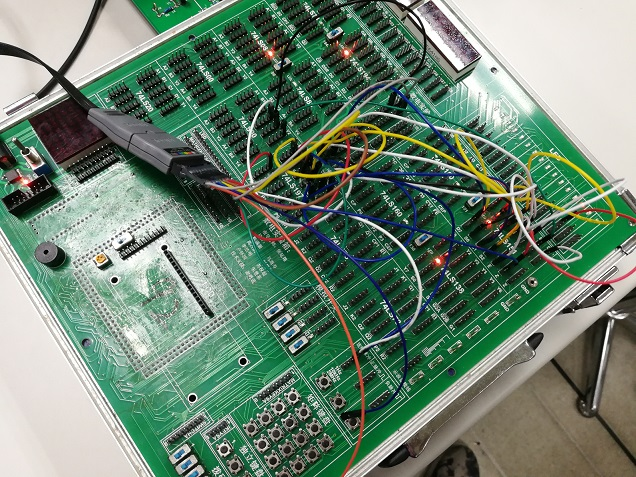
\includegraphics[width=0.5\linewidth]{fig/p1.jpg}&
    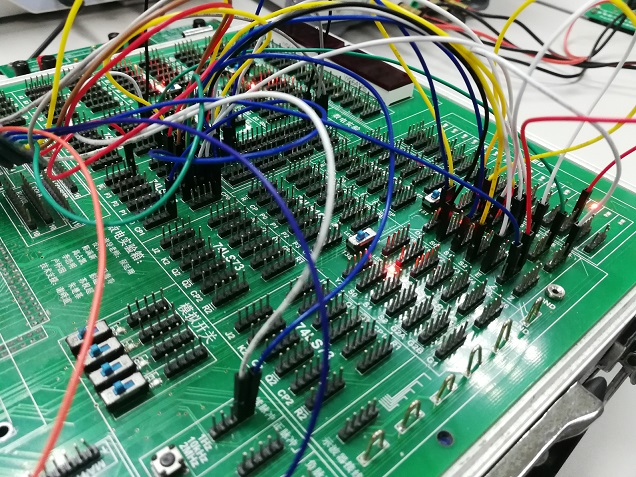
\includegraphics[width=0.5\linewidth]{fig/p1-1.jpg}
    \end{tabular}
\end{figure}
\par 波形图如下
\begin{figure}[H]
    \centering
    \includegraphics[width=0.6\linewidth]{fig/DS2_QuickPrint1.png}
\end{figure}
\par 可以明显看出当输入$S2,S1,S0$每八个一循环时,$\overline{G1}$也依次在不同的位置输出


% 90 W5 分频自己跑1Hz
\section{内容二}
\subsection{实验目的}
实现一个逻辑单元(LU, Logic Unit)

\subsection{实验原理}
逻辑单元功能如下
% Table generated by Excel2LaTeX from sheet 'Sheet3'
\begin{table}[H]
  \centering
    \begin{tabular}{|c|c|c|}
    \hline
    M1    & M0    & Y \bigstrut\\
    \hline
    0     & 0     & AB \bigstrut\\
    \hline
    0     & 1     & A+B \bigstrut\\
    \hline
    1     & 0     & A$\oplus$B \bigstrut\\
    \hline
    1     & 1     & $\overline{A}$ \bigstrut\\
    \hline
    \end{tabular}%
  \label{tab:addlabel}%
\end{table}%
\par 真值表如下
% Table generated by Excel2LaTeX from sheet 'Sheet2'
\begin{table}[H]
  \centering
    \begin{tabular}{|c|c|c|c|c|r|c|c|c|c|c|}
\cline{1-5}\cline{7-11}    M1    & M0    & A     & B     & Y     &       & M1    & M0    & A     & B     & Y \bigstrut\\
\cline{1-5}\cline{7-11}    0     & 0     & 0     & 0     & 0     &       & 1     & 0     & 0     & 0     & 0 \bigstrut\\
\cline{1-5}\cline{7-11}    0     & 0     & 0     & 1     & 0     &       & 1     & 0     & 0     & 1     & \textcolor[rgb]{ 1,  0,  0}{1} \bigstrut\\
\cline{1-5}\cline{7-11}    0     & 0     & 1     & 0     & 0     &       & 1     & 0     & 1     & 0     & \textcolor[rgb]{ 1,  0,  0}{1} \bigstrut\\
\cline{1-5}\cline{7-11}    0     & 0     & 1     & 1     & \textcolor[rgb]{ 1,  0,  0}{1} &       & 1     & 0     & 1     & 1     & 0 \bigstrut\\
\cline{1-5}\cline{7-11}    0     & 1     & 0     & 0     & 0     &       & 1     & 1     & 0     & 0     & \textcolor[rgb]{ 1,  0,  0}{1} \bigstrut\\
\cline{1-5}\cline{7-11}    0     & 1     & 0     & 1     & \textcolor[rgb]{ 1,  0,  0}{1} &       & 1     & 1     & 0     & 1     & \textcolor[rgb]{ 1,  0,  0}{1} \bigstrut\\
\cline{1-5}\cline{7-11}    0     & 1     & 1     & 0     & \textcolor[rgb]{ 1,  0,  0}{1} &       & 1     & 1     & 1     & 0     & 0 \bigstrut\\
\cline{1-5}\cline{7-11}    0     & 1     & 1     & 1     & \textcolor[rgb]{ 1,  0,  0}{1} &       & 1     & 1     & 1     & 1     & 0 \bigstrut\\
\cline{1-5}\cline{7-11}    \end{tabular}%
\end{table}%
\par 将S2,S1,S0分别与输入Q3,Q2,Q1相连,作为M1,M0,A;Q0依据一定规则与数据输入端相连,作为B;即输出是通过比较B与Y的异同决定.
\par 分析表格,并由数字选择器的原理可知$D0,D7=0$,$D1,D2,D4=Q0$,$D3,D6=1$,$D5=\overline{Q0}$

\subsection{实验细节}
\subsubsection{实验仪器及器件}
\begin{enumerate}
    \item 数字电路实验箱、示波器、导线若干
    \item 74LS151*1, 74LS197*1
\end{enumerate}

\subsubsection{Protues电路设计及仿真}
设计电路如下
\begin{figure}[H]
    \centering
    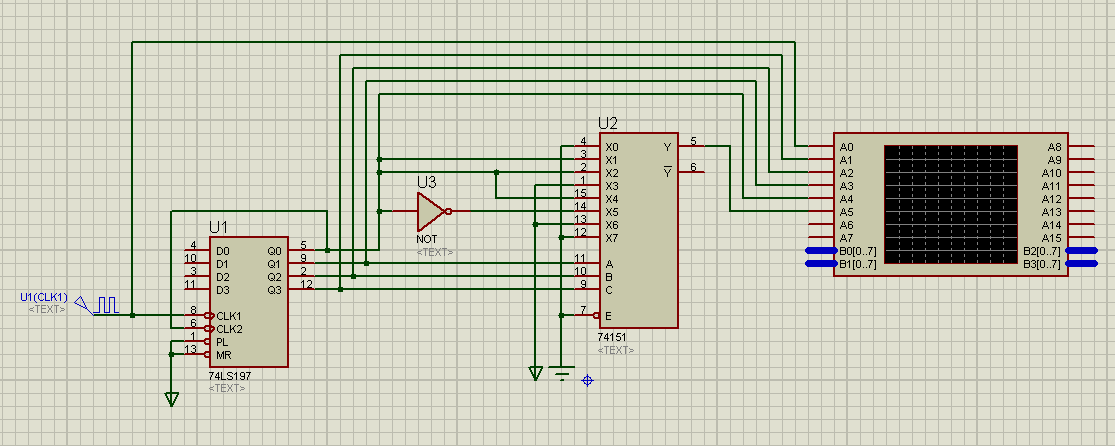
\includegraphics[width=0.9\linewidth]{fig/74151.PNG}
\end{figure}
\par 示波器的A0,A1,A2,A3,A4,A5分别对应CP,M1,M0,A,B,Y,结果波形图如下
\begin{figure}[H]
    \centering
    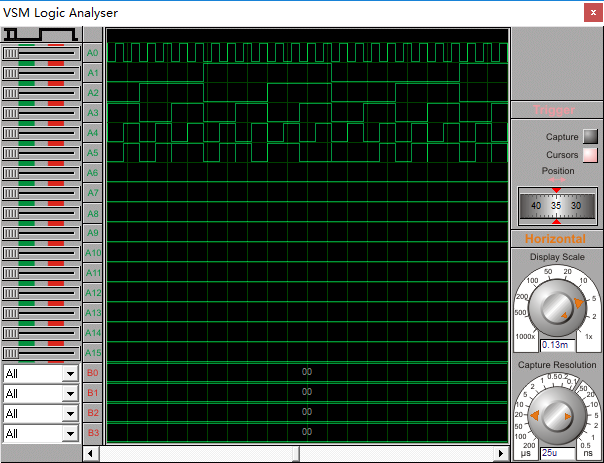
\includegraphics[width=0.5\linewidth]{fig/74151_wave.PNG}
\end{figure}

\subsubsection{实验流程}
\begin{enumerate}
    \item 将74LS197连接成十六进制作为电路的输入信号源:$\overline{PL}$,$\overline{MR}$接高电平,CP0接时钟输入
    \item 74LS151的连线与Protues仿真示例相同
    \item 用示波器观测并记录CP,M1,M0,A,B,Y的波形
\end{enumerate}

\subsection{结果分析及结论}
\par 静态测试:接01显示器显示正常
\par 动态测试:实验箱连线如下
\begin{figure}[H]
    \centering
    \begin{tabular}{cc}
    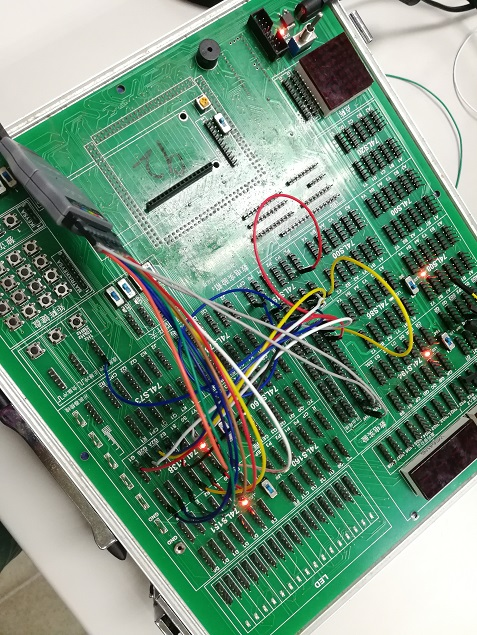
\includegraphics[width=0.4\linewidth]{fig/p2.jpg}&
    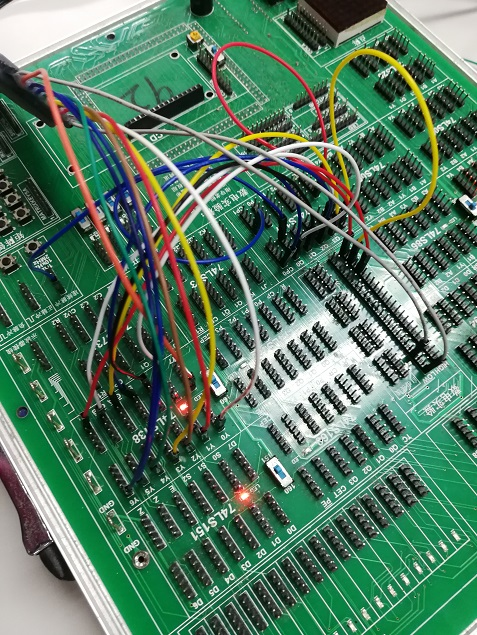
\includegraphics[width=0.4\linewidth]{fig/p2-1.jpg}
    \end{tabular}
\end{figure}
\par 波形图如下
\begin{figure}[H]
    \centering
    \includegraphics[width=0.6\linewidth]{fig/DS2_QuickPrint2.png}
\end{figure}
\par 由波形图可见,符合逻辑单元的要求输出

\subsection{Bayse板电路实现}
\par Verilog程序如下,LU单元
\begin{lstlisting}[language=Verilog]
module LU (
    input wire [1:0] op,
    input wire A,
    input wire B,
    output reg res
    );
    
    always @(*) begin
    case (op)
        2'b00: res <= A & B;
        2'b01: res <= A | B;
        2'b10: res <= A^B;
        2'b11: res <= ~A;
    endcase
    end

endmodule
\end{lstlisting}
\par 16进制分频计数器
\begin{lstlisting}[language=Verilog]
// 100MHz -> 1Hz
module Counter(
    input wire clr, // clear, say reset
    input wire clk, // clock
    output reg [3:0] out // 4 bits output
    );

    // time counter
    localparam MAX_COUNT = 50_000_000; // 0.5s
    reg [25:0] count; // 26 bits to store count: 2^26 > 5*10^7
    always @ (posedge clk or posedge clr)
    begin
        if (clr == 1) // reset
            count <= 0;
        else if (count == MAX_COUNT - 1) // return 0
            count <= 0;
        else
            count <= count + 1;
    end

    // frequency divisor (flip-flop)
    reg clk_div;
    always @ (posedge clk, posedge clr)
    begin
        if (clr == 1)
            clk_div <= 0;
        else if (count == MAX_COUNT - 1) // reset
            clk_div <= ~clk_div;
        else // set
            clk_div <= clk_div;
    end

    // hex counter
    always @ (posedge clk_div, posedge clr)
    begin
        if (clr == 1)
            out <= 0;
        else if (clk_div == 1)
            out <= out + 1;
        else
            out <= out;
    end

endmodule
\end{lstlisting}
\par 顶层封装
\begin{lstlisting}[language=Verilog]
module wrapper (
    input clk,
    output wire A,
    output wire B,
    output wire [1:0] op_code,
    output wire res
    );
    
    wire [2:0] out;
    Counter Counter(.clr(clr), .clk(clk), .out({op_code, A, B}));
    LU LU(.op(op_code), .A(A), .B(B), .res(res));

endmodule
\end{lstlisting}
\par Vivado内模拟仿真如下
\begin{figure}[H]
    \centering
    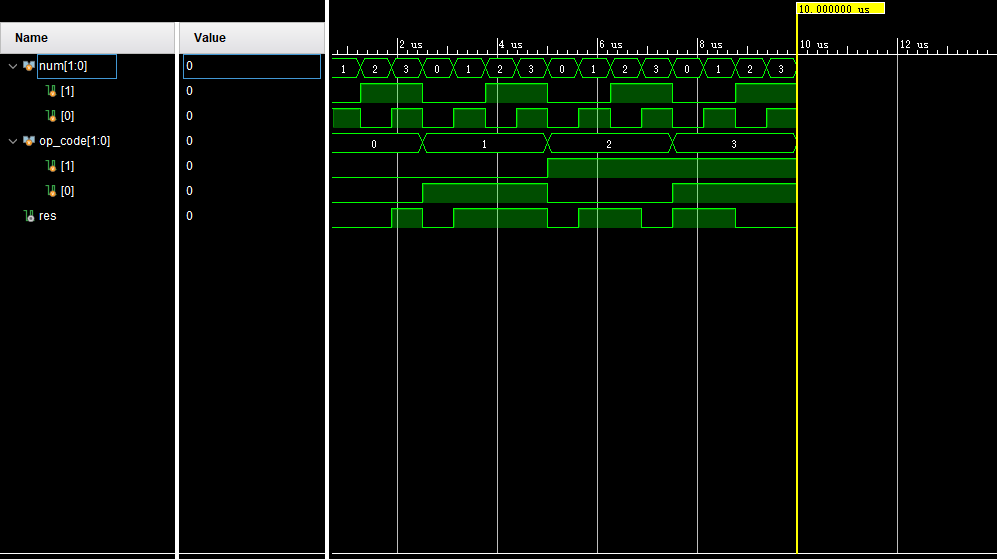
\includegraphics[width=0.6\linewidth]{fig/vivado_wave.PNG}
\end{figure}
\par 由于无法放入动态图,故只放一张静态图,如下,LD15,LD14,LD13,LD12,LD11分别为M1,M0,A,B,Y
\begin{figure}[H]
    \centering
    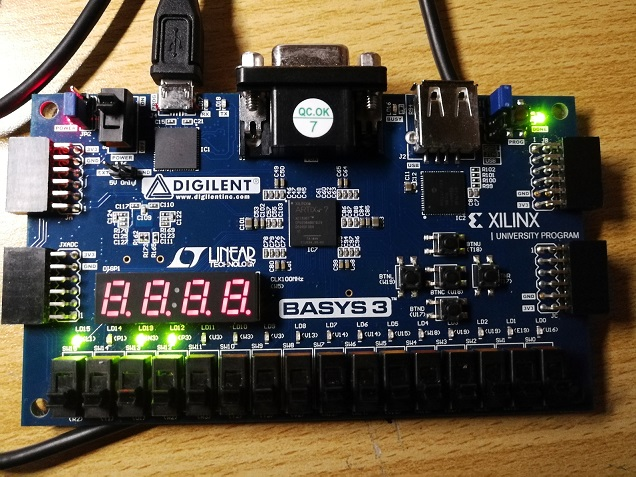
\includegraphics[width=0.6\linewidth]{fig/board.jpg}
\end{figure}


\section{内容三}
\subsection{实验目的}
实现一个算术单元(AU, Arithmetic Unit)--半加半减器

\subsection{实验原理}
\par 真值表如下所示
% Table generated by Excel2LaTeX from sheet 'Sheet4'
\begin{table}[H]
  \centering
    \begin{tabular}{|c|c|c|c|c|}
    \hline
    M     & A     & B     & Y     & C \bigstrut\\
    \hline
    0     & 0     & 0     & 0     & 0 \bigstrut\\
    \hline
    0     & 0     & 1     & \textcolor[rgb]{ 1,  0,  0}{1} & 0 \bigstrut\\
    \hline
    0     & 1     & 0     & \textcolor[rgb]{ 1,  0,  0}{1} & 0 \bigstrut\\
    \hline
    0     & 1     & 1     & 0     & \textcolor[rgb]{ 1,  0,  0}{1} \bigstrut\\
    \hline
    1     & 0     & 0     & 0     & 0 \bigstrut\\
    \hline
    1     & 0     & 1     & \textcolor[rgb]{ 1,  0,  0}{1} & \textcolor[rgb]{ 1,  0,  0}{1} \bigstrut\\
    \hline
    1     & 1     & 0     & \textcolor[rgb]{ 1,  0,  0}{1} & 0 \bigstrut\\
    \hline
    1     & 1     & 1     & 0     & 0 \bigstrut\\
    \hline
    \end{tabular}%
\end{table}%
\par 由表可立得Y和C的表达式,以乘积之和(SOP)的形式表示
\[Y=m_{1,2,5,6},C=m_{3,5}\]
\par 由于这种形式可直接得到数据选择器或数据分配器的连线方式,故不需用卡诺图进行构造化简

\subsection{实验细节}
\subsubsection{实验仪器及器件}
\begin{enumerate}
    \item 数字电路实验箱、示波器、导线若干
    \item 74LS197*1
    \item 74LS151*2或74LS138*1+74LS20*2
\end{enumerate}

\subsubsection{实验流程}
\begin{enumerate}
    \item 将74LS197连接成十六进制作为电路的输入信号源:$\overline{PL}$,$\overline{MR}$接高电平,CP0接时钟输入
    \item 第一个74LS151的S2,S1,S0分别接Q2,Q1,Q0,D1,D2,D5,D6接高电平,其余接低电平;\\
    第二个74LS151的S2,S1,S0分别接Q2,Q1,Q0,D3,D5接高电平,其余接低电平
    \item 或者74LS138的$\overline{G2A}$,$\overline{G2B}$接低电平,G1接高电平,Y1,Y2,Y5,Y6接第一个与非门(74LS20)输出Y,Y3,Y5接第二个与非门输出C
    \item 用示波器观测并记录CP,M,A,B,Y,C的波形
\end{enumerate}

\subsection{结果分析及结论}
\par 静态测试:接01显示器显示正常
\par 动态测试:实验箱连线如下
\begin{figure}[H]
    \centering
    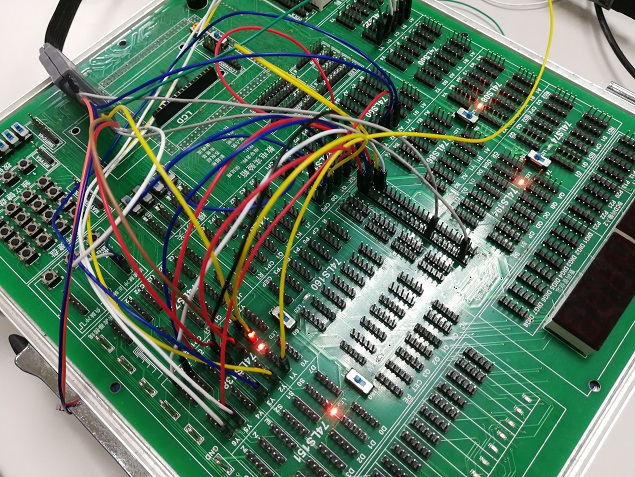
\includegraphics[width=0.6\linewidth]{fig/p3.jpg}
\end{figure}
\par 波形图如下
\begin{figure}[H]
    \centering
    \includegraphics[width=0.6\linewidth]{fig/DS2_QuickPrint3.png}
\end{figure}
\par 由波形图可见,符合算术单元的要求输出

\begin{comment}
\section{内容四-1}
\subsection{实验目的}
用Vivado在Basys3实验板上实现一个六输入二输出的1Bit算术逻辑单元(ALU, Arithmetic \& Logic Unit)

\subsection{实验原理}
六个输入包括三个控制端和三个数据输入端
\begin{enumerate}
    \item 控制端:S2,S1,S0决定ALU的8种功能,如下表所示\\
    % Table generated by Excel2LaTeX from sheet 'Sheet5'
\begin{table}[H]
  \centering
    \begin{tabular}{|c|c|c|c|}
    \hline
    S2    & S1    & S0    & 功能 \bigstrut\\
    \hline
    0     & 0     & 0     & 与 \bigstrut\\
    \hline
    0     & 0     & 1     & 或 \bigstrut\\
    \hline
    0     & 1     & 0     & 非A \bigstrut\\
    \hline
    0     & 1     & 1     & 非B \bigstrut\\
    \hline
    1     & 0     & 0     & 异或 \bigstrut\\
    \hline
    1     & 0     & 1     & 全加 \bigstrut\\
    \hline
    1     & 1     & 0     & 全减 \bigstrut\\
    \hline
    1     & 1     & 1     & 清零 \bigstrut\\
    \hline
    \end{tabular}%
\end{table}%
    \item 数据输入端:\\
    当ALU进行全加(全减)运算时,三个数据输入端分别为被加数(被减数)、加数(减数)、进位(借位);\\
    当ALU进行逻辑运算(与、或、非、异或)时,三个数据输入端中的两个作为操作数的输入,另外一个可以忽略
    \item 输出端:\\
    当ALU进行全加(全减)运算时,两个输出端分别为和(差)、进位(借位);\\
    当ALU进行逻辑运算时,两个输出端为逻辑运算的结果和结果的取反
\end{enumerate}
其中,全加器(左)和全减器(右)的真值表如下
% Table generated by Excel2LaTeX from sheet 'Sheet6'
\begin{table}[H]
  \centering
    \begin{tabular}{|c|c|c|c|c|r|c|c|c|c|c|}
\cline{1-5}\cline{7-11}    A     & B     & C     & SUM   & CARRY &       & A     & B     & C     & DIFF  & CARRY \bigstrut\\
\cline{1-5}\cline{7-11}    0     & 0     & 0     & 0     & 0     &       & 0     & 0     & 0     & 0     & 0 \bigstrut\\
\cline{1-5}\cline{7-11}    0     & 0     & 1     & \textcolor[rgb]{ 1,  0,  0}{1} & 0     &       & 0     & 0     & 1     & \textcolor[rgb]{ 1,  0,  0}{1} & \textcolor[rgb]{ 1,  0,  0}{1} \bigstrut\\
\cline{1-5}\cline{7-11}    0     & 1     & 0     & \textcolor[rgb]{ 1,  0,  0}{1} & 0     &       & 0     & 1     & 0     & \textcolor[rgb]{ 1,  0,  0}{1} & \textcolor[rgb]{ 1,  0,  0}{1} \bigstrut\\
\cline{1-5}\cline{7-11}    0     & 1     & 1     & 0     & \textcolor[rgb]{ 1,  0,  0}{1} &       & 0     & 1     & 1     & 0     & \textcolor[rgb]{ 1,  0,  0}{1} \bigstrut\\
\cline{1-5}\cline{7-11}    1     & 0     & 0     & \textcolor[rgb]{ 1,  0,  0}{1} & 0     &       & 1     & 0     & 0     & \textcolor[rgb]{ 1,  0,  0}{1} & 0 \bigstrut\\
\cline{1-5}\cline{7-11}    1     & 0     & 1     & 0     & \textcolor[rgb]{ 1,  0,  0}{1} &       & 1     & 0     & 1     & 0     & 0 \bigstrut\\
\cline{1-5}\cline{7-11}    1     & 1     & 0     & 0     & \textcolor[rgb]{ 1,  0,  0}{1} &       & 1     & 1     & 0     & 0     & 0 \bigstrut\\
\cline{1-5}\cline{7-11}    1     & 1     & 1     & \textcolor[rgb]{ 1,  0,  0}{1} & \textcolor[rgb]{ 1,  0,  0}{1} &       & 1     & 1     & 1     & \textcolor[rgb]{ 1,  0,  0}{1} & \textcolor[rgb]{ 1,  0,  0}{1} \bigstrut\\
\cline{1-5}\cline{7-11}
 \end{tabular}%
\end{table}%
\par 注:ALU的输入端接6位计数器的输出


\subsection{实验细节}

\subsection{结果分析及结论}
此处应有图


\section{内容四-2}
\subsection{实验目的}
用Vivado在Basys3实验板上实现一个十二输入二输出的4Bit算术逻辑单元

\subsection{实验原理}
十二个输入包括三个控制端M2,M1,M0和九个数据输入端A,B,Cn,A1,B1,A2,B2,A3,B3,功能与1Bit的ALU相同

\subsection{实验细节}

\subsection{结果分析及结论}
此处应有图
\end{comment}

\end{document}
% 实验目的
% 原理
% 所用仪器及器件
% 实验内容
%% 设计流程
%% proteus电路设计和仿真
%% 实验箱电路静态、动态测试步骤和结果
%% 相关分析说明
% 结论